%!TEX root = ../main.tex
\section{Evaluation}
\label{sec: evaluation}
We now present the evaluation of our \textit{Assisted I/O library} and \textit{Advice Manager} prototypes with a real world application used by physicists at the data processing center of the University of Mainz (ZDV). Our testbed is composed by %two separate systems: 
a test cluster of seven nodes, mainly intended to evaluate the proposed Linux kernel modification with the Lustre file system. %, and the Mogon cluster, currently the production system at the ZDV. 
We start with a concise description of the %two 
system as well as a detailed analysis of the target application's I/O pattern, and then present the results of our experiments. 

We evaluate the performance of our framework using two metrics, the execution time of the test application and the number of reads completed by every target file system. %To simulate a heavily loaded cluster we use a background process that runs on an set of nodes independent from the node running the target application. Additionally, we also measure the overhead introduced by our prototype. 

\subsection{Test Cluster}
\label{subsec: test_cluster}
%As already mentioned, this small cluster is aimed mainly to test our modified kernel with Lustre. The reason is that it was not possible to disrupt the production cluster, affecting hundreds of users, by re-installing the operating system kernel. 
%In order to make realistic comparisons between Lustre and GPFS, the test cluster also mounts a GPFS file system. The only GPFS network shared disk (NSD) servers and Lustre object storage servers (OSS) are hosted by two machines (DELL R710 equipped with two quadcore E5620 @ 2.4GHz and 24GB main memory) of the seven available. The disk setup consists of one DELL MD3200 and four MD1200, connected to the two storage servers in a failover configuration. Each of the storage enclosures is equipped with 12 disks (for a total of 60 disks) and configured with 8+2 RAID 6 (6 8+2 RAIDs in total). Four of the six available RAIDs are used as Lustre OSTs and GPFS NSDs (with separated partitions). The Lustre MDS is hosted by a SuperMicro Chassis equipped with one quadcore Xeon E3-1230 @ 3.3GHz and 16GB of main memory. In this case the metadata target (MDT) is a 120 GB SSD Intel 520. The remaining four machines, equipped with an eight core E3-1230 @ 3.3GHz processor and 24 GB of main memory, work as compute nodes and file system clients. All of the machines are connected to a 24 ports SSE-245 Gbit ethernet switch. Both the GPFS and Lustre file systems are formatted with a block size of 4MB.

%Markus description
As already mentioned, this small cluster is aimed mainly to test our modified kernel with Lustre. 
The reason is that it was not possible to disrupt the production cluster, affecting hundreds of users, by re-installing the operating system kernel.
In order to make realistic comparisons between Lustre and GPFS, the test cluster also has a GPFS file system on comparable hardware. 
Both filesystems have a single disk server each, one Dell R710 acts as GPFS network shared disk (NSD) server and another as Lustre object storage server (OSS). The R710 are equipped with two quadcore E5620 @ 2.4GHz and 24GB main memory. For storage, both disk servers share a MD3200 array with 2 controllers and 4 MD1200 expansion shelves for a total of 60 2TB drives. The Storage is formatted in 4 15 dynamic disk pools. This is the LSI/Netapp type of declustered RAID, which distributes the 8+2 RAID6 stripes evenly over all 15 disks for better rebuild performance. The disk block size is set to 128KiB, which results in a RAID stripe size of 1MiB. The four disk pools are then split on the Array into LUNs, one of the LUNs from each disk pool is then used for GPFS and another one from each pool is used for Lustre. This results in comparable resources for both filesystems and tests do not interfere with each other, as long as only one filesystem is tested at a time. While the GPFS filesystem embeds the metadata with the data, Lustre needs a separate Metadata Server (MDS). This is hosted by a SuperMicro server equipped with one quadcore Xeon E3-1230 @3.3GHz and 16GB of main memory, as metadata target (MDT) it uses a 120GB SSD Intel 520. Four other machines of the same type, equipped with an eight core E3-1230 @3.3GHz processor and 16GB of main memory, work as compute nodes and file system clients. All machines, servers and clients, are equipped with Intel X520DA 10Gigabit adapters and connected to a SuperMicro SSE-X24S 24 ports 10 Gigabit switch. Both, the GPFS and Lustre file systems are formatted with a block size of 4MB.
%The Lustre file system was formatted with a block size of 4MB. It is composed of 4 OSTs and a MDT.%; the input files we used were belonging each one to a different OSTs. %We also tried to stripe the files over all the OSTs, but didn't notice any difference in the execution times.

%GPFS was also formatted with a block size of 4MB and has 4 NSDs.
 
%\subsection{Production Cluster}
%\%label{subsec: mogon}
%The Mogon cluster has 535 nodes each equipped with four 16 core CPUs @ 2.1GHz processors for a total of 34,240 cores. All of the nodes run the Scientific Linux distribution with kernel version `2.6.32-358.2.1.el6.x86\_64' and are connected via QDR Infiniband network. The native parallel file system is GPFS, formatted with a block size of 4MB like the one in the test cluster. Mogon has eleven GPFS NSD servers serving three separate file systems. We chose one of them to conduct our experiments. We reserved a full node (i.e. 64 cores) via the LSF batch system, specifying 2GB of memory for each core.

%The connection between the nodes is Infiniband. %that if necessary can fall back to RDMA if something is wrong.
% TODO: what sort of Infiniband? Probably 'QDR'?
%GPFS is the native parallel file system in Mogon and therefore we were able to run our advice infrastructure prototype already installed in the production cluster so we were able to test our framework on Mogon. Each node provides 1.5$\,$TB of local disk space, which gave us the possibility to test the ext4 file system in one of these nodes.

\subsection{Real World Application}
\label{subsec: application}
Our target real world application is written using `ROOT', an object-oriented framework widely adopted in the experimental high energy physics community to build software for data analysis. The application analyzes data read from an input file in the `ROOT' format (structured file format). %The file we used is 5GB in size.

\begin{figure}[!htb]
  \centering
  \begin{subfigure}[t]{\columnwidth}
    \centering
    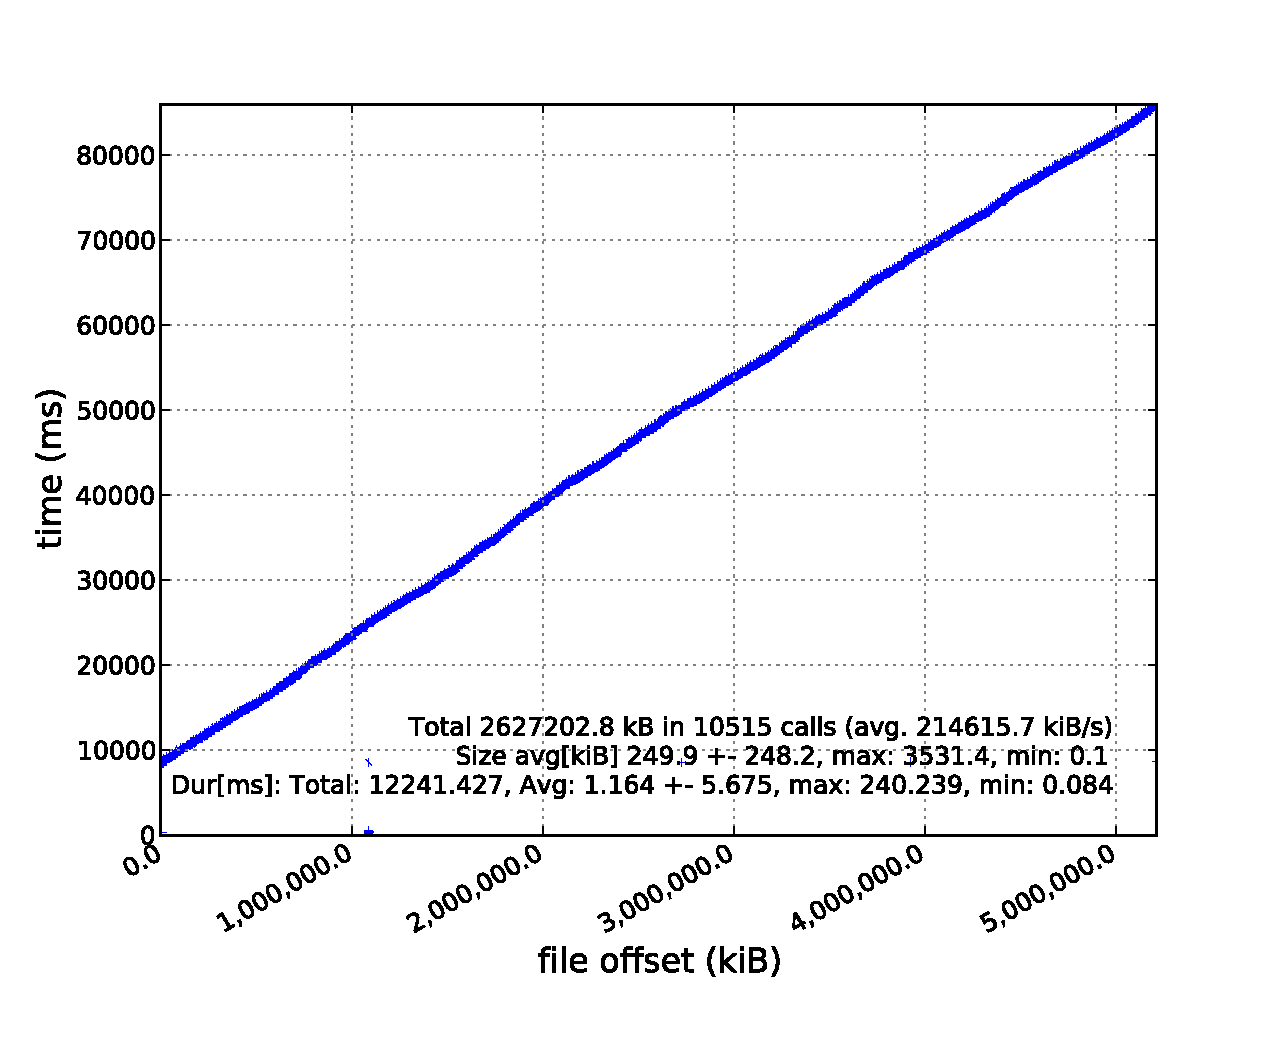
\includegraphics[width=\columnwidth]{figures/iopat_profile}
    \caption{\textit{}}
    \label{figure: iopat_profile}
  \end{subfigure}
  \begin{subfigure}[t]{\columnwidth}
    \centering
    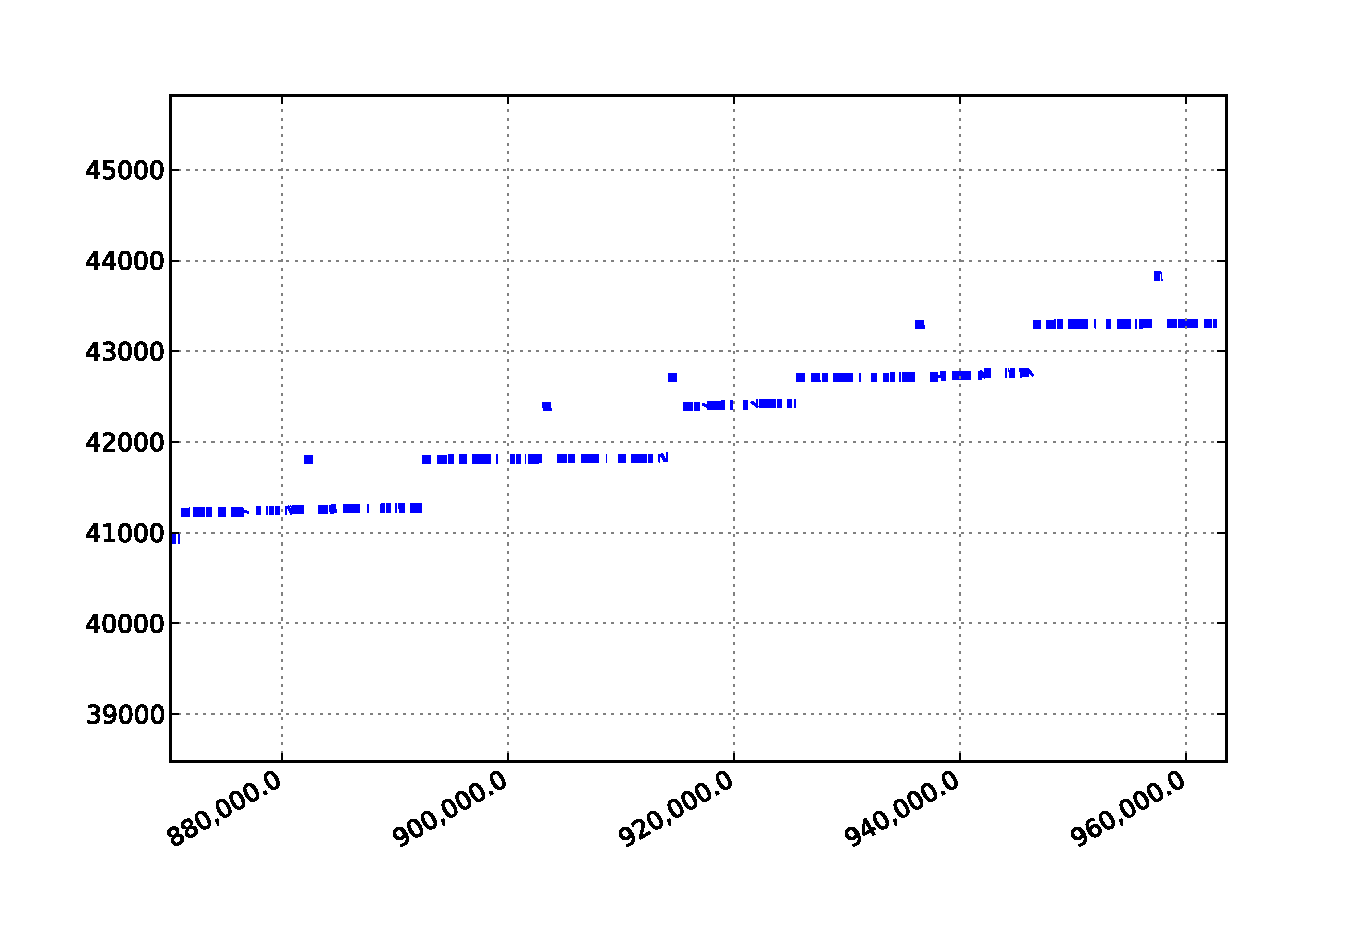
\includegraphics[width=\columnwidth]{figures/00050_zoom}
    \caption{\textit{}}
    \label{figure: iopat_zoom}
  \end{subfigure}
  \caption{I/O read profile of the target application under analysis (\ref{figure: iopat_profile}), extracted from the the GPFS file system in the test cluster, and zoomed window (\ref{figure: iopat_zoom}) showing the actual pattern details.}
  \label{figure: iopattern_with_statistics}
\end{figure}

First of all we characterized the application's I/O pattern for a target file using traces and statistics extracted through several tools such as \textit{strace}, \textit{ioapps}~\cite{ioapps} and GPFS's \textit{mmpmon}~\cite{mmpmon} monitoring tool. Figure~\ref{figure: iopattern_with_statistics} shows the I/O pattern along with some additional statistics. As it can be seen, in this specific case (5GB file), the application issues a total of 10515 \texttt{read()} system calls to read about 2.6GB of total data. The average request size is 250kiB and the time spent waiting for I/O is 12 seconds, when running on the test cluster. 

At a first glance the general I/O behaviour of the application looks linear, most of the accesses to the file follow an increasing offset. Nevertheless, adjacent reads are separated by gaps (a strided read pattern). In a few cases this gap becomes negative, meaning that the application is moving backwards in the file to read some data previously left behind (as reported in Figure~\ref{figure: iopat_zoom}). %(Figure~\ref{figure: 00050_zoom}). 

%\begin{figure}[!htb]
%  \centering
%  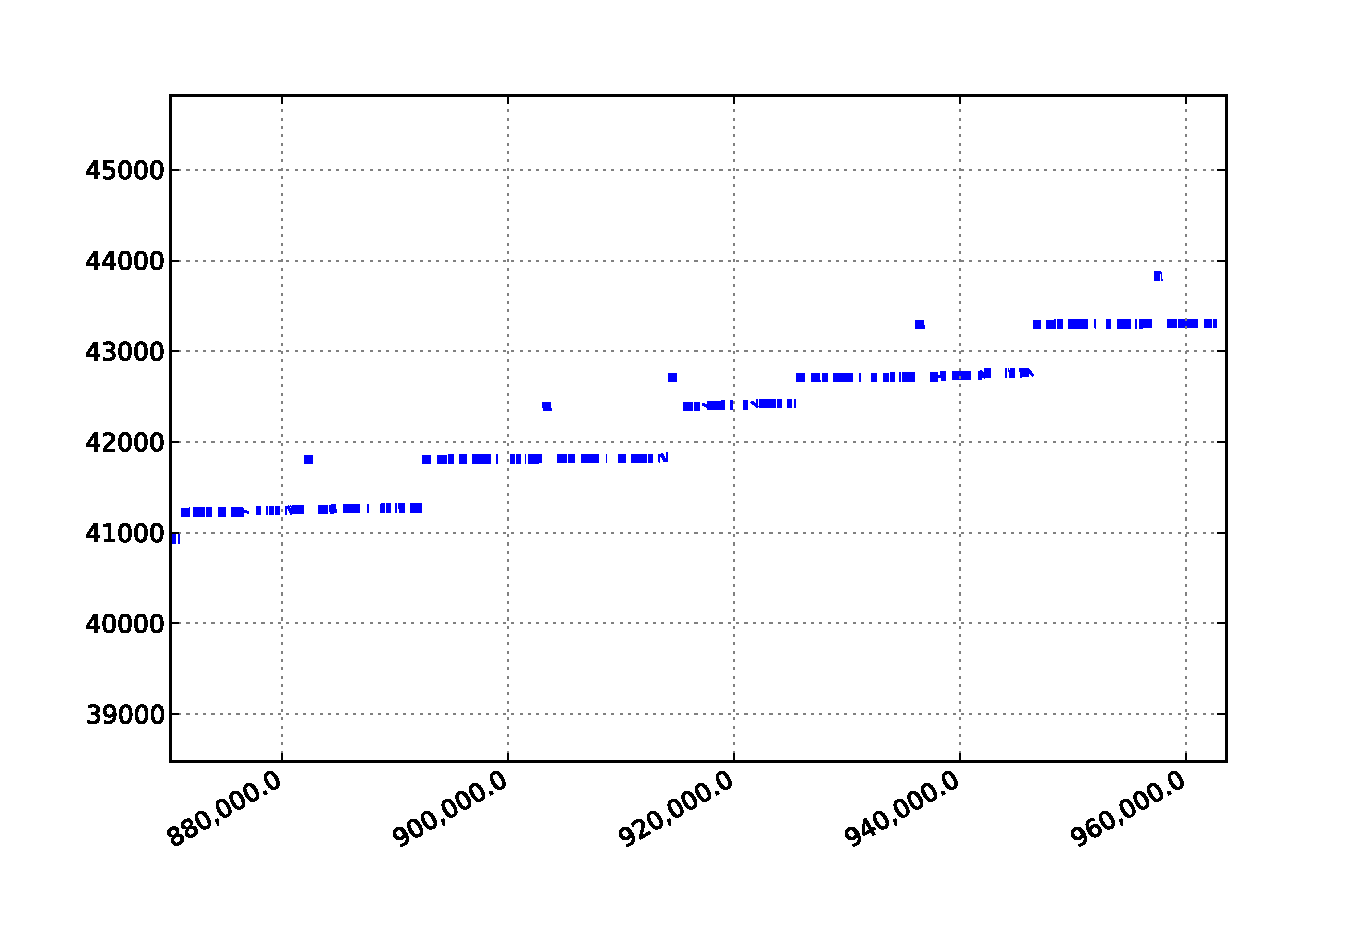
\includegraphics[width=0.44\textwidth]{figures/00050_zoom}
%  \caption{Zoomed version of the I/O pattern under analysis. Here backwards seeks are clearly visible.}
%  \label{figure: 00050_zoom}
%\end{figure}

After a detailed I/O pattern analysis we could divide the target file into contiguous non overlapping ranges. Within these ranges reads happen to have increasing offset. %The information extracted was then used to tailor a configuration file of the form described in Listing~\ref{config}, with each discovered range forming a part of the `WillNeed' section. 
Even though the general I/O pattern of the application for different files looks similar\footnote{Due to space limits we do not report the comparison between different files.}, the size of the non overlapping ranges may change significantly. This general behaviour can be modelled using a configuration file in which a `WillNeed' hint covers the whole file from beginning to end (i.e. `Offset' and `Length' equal to 0). The backwards seeks can be accounted for using the `CacheSize' parameter to keep previously accessed blocks in cache. In this way we effectively emulate a sliding window that tracks the application's I/O behaviour. This would not be possible by just using a, e.g., \texttt{POSIX\_FADV\_WILLNEED} advice on the whole file before starting the application like shown by Figure~\ref{figure: fadvise_comparison}. The reason is that if the file size is equal or smaller than the cache size, we would have a large number of valuable pages discarded from the cache to load data that will be accessed at the end of the application. Additionally, if the file size is bigger than the cache size we would have the file system discarding blocks at the beginning of the file as the blocks at the end are preloaded, effectively forcing the application to access these blocks from the I/O servers instead of the cache. With our approach, on the other hand, we keep in the cache only a small, controlled number of blocks (the ones currently accessed), while the older blocks are discarded since no longer needed. %For GPFS this causes an over-specialized configuration file to be generated, that works in one case less effectively than in another. The reason is that GPFS requires the user to release all the hints that have been previously acquired. If the \textit{Advisor Threads} uses a configuration file that does not match the current I/O pattern, prefetched blocks may be released and afterwards accessed again by the application causing a cache miss. For POSIX advice this is not an issue as the API does not require the releasing of prefetched ranges\footnote{This choice was imposed by the fact that \texttt{POSIX\_FADV\_DONTNEED} can be quite time consuming and its employment can considerably slow down the `Advisor Thread', making it useless.}.
% and leave instead the duty to the LRU algorithm in the page cache. In any case, the configuration file mechanism is flexible and users with specific requirements can easily add support for their I/O patterns, improving the performance of their applications.

\begin{figure}[!htb]
  \centering
  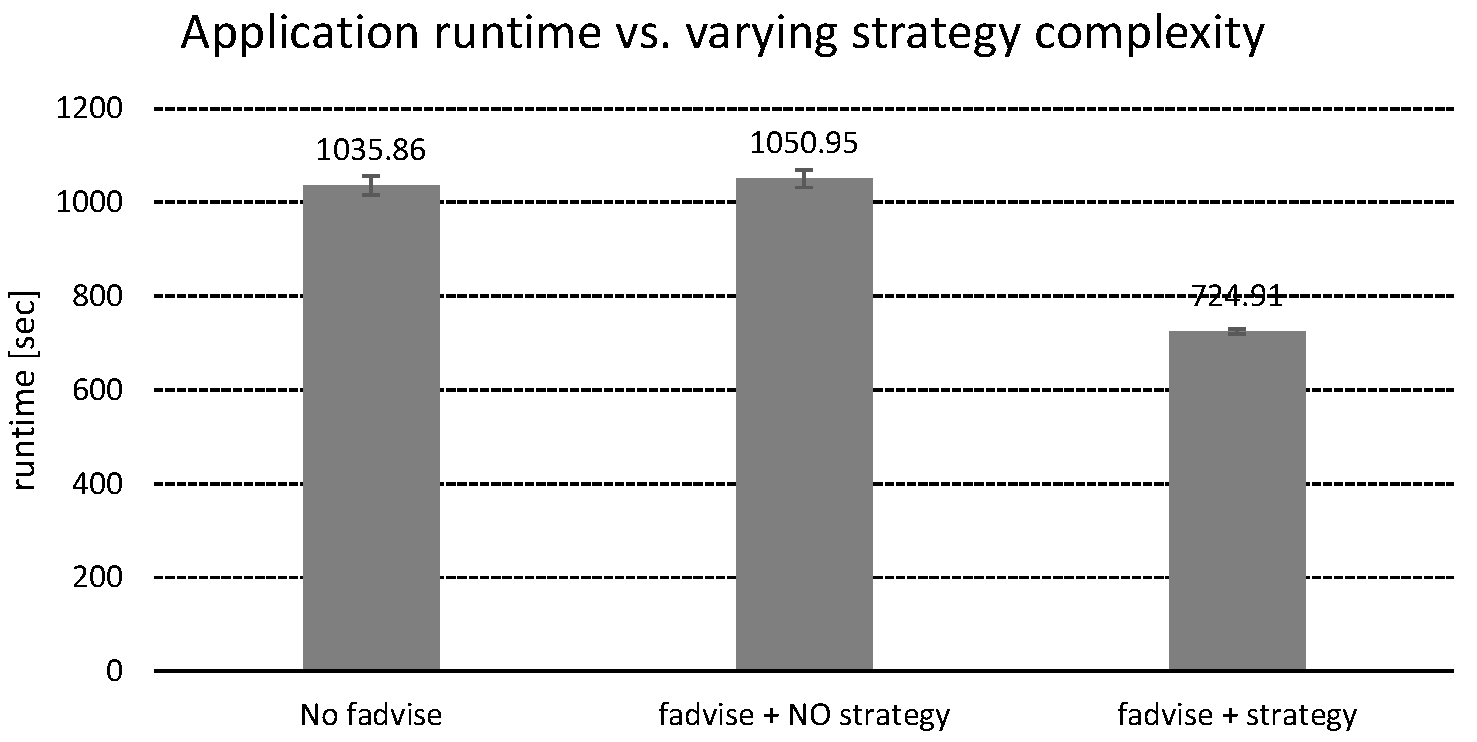
\includegraphics[width=\columnwidth]{figures/SC2015/ROOT/separate_plots/test_cluster/test_fadvise_no_border}
  \caption{Comparison between different usage stategies of posix\_fadvise for an input file of 55GB residing in an ext4 file system. The first bar represents the case in which no advice is used, the second bar represents the case in which a POSIX\_FADV\_WILLNEED is issued for the whole file at the beginning of the application and the third bar represents the case in which POSIX\_FADV\_WILLNEED is issued using MERCURY.}
  \label{figure: fadvise_comparison}
\end{figure} 
 
To assess the impact of our prototype on the application and file systems performance we considered the application execution time and the number of reads accounted for by the respective file systems. We conducted our experiments without file system hints and then with file system hints issued transparently to the application by the \textit{Advice Manager}. Furthermore, we ran each experiment three times and calculated average, minima and maxima for each metric. In order to avoid caching affecting our measurements, extra care was taken to clean all the relevant caches for the different file systems. For ext4 and Lustre this was accomplished by using the command line: $$echo\ 3 > /proc/sys/vm/drop\_caches$$ on the file system clients. Additionally, for Lustre this command was also executed on the OSS to avoid the server side cache to be retained. In the case of GPFS, the file system client's page pool was cleaned using the clean file cache hint in Table~\ref{table: hints_table}, the NSD servers do not cache any data. 
% unmounting the file system and remounting it again. %TODO: is this quoting a GPFS manual?
%On the Mogon cluster we could not unmount and shutdown GPFS, so we cleaned the client page pool as mentioned before. We checked using the test cluster that the effect of the missing steps (shutting down GPFS and unmounting it) did not have any effect on our results.

\subsection{Execution Time}
\label{subsec: results}
To measure the performance improvements that our prototype can deliver to the application's runtime we conducted two set of tests. In the first test we varied the size of the input file from 5 to 95GB. This is mainly aimed to study the behaviour of the `ROOT' application using different input file sizes and how our solution behaves when the file becomes bigger than the available cache space. In the second test we varied the number of `ROOT' instances running simultaneously from 1 to 8. By doing so we study the interaction of multiple processes accessing the file system and how these can benefit from the prefetching hints generated by MERCURY. Figure~\ref{figure: runtime} reports the results for the described experiments. All the tests where performed using a `BlockSize' of 4MB, a `CacheSize' of 8 blocks, a `ReadAheadSize' of 4 blocks, and a `WillNeed' hint covering the whole file (i.e. with `Offset' and `Length' equal to 0), resulting in each process consuming up to 32MB of cache space and 512MB in total for 8 application instances. The `WillNeed' on the whole file causes the \textit{Advisor Thread} to issue up to 4 (`ReadAheadSize') prefetching requests for blocks of 4MB sequentially, starting from the current accessed block. This has the same effect of data sieving in ROMIO, optimizing the access size and allowing the application to read the requested data randomly from the cache instead of the file system. The produced effect is particularly beneficial in the case of Lustre and ext4, as it can be seen in Figures~\ref{figure: ext4_1} and~\ref{figure: lustre_1}. In these cases we measure reductions in the execution time of up to 50\% circa, with respect to the normal case. For GPFS we can still observe an improvement but this is more contained compared to the other file systems (Figure~\ref{figure: gpfs_1}). The reductions in the execution time measured in GPFS are on average up to 10\%, with respect to the normal case. The reason is that the default prefetching strategy in GPFS works better that traditional read-ahead. In fact, by disabling the prefetching in GPFS we observed reductions in the execution time comparable to the other file systems (not reported here).
\begin{figure*}[!htb]
  \centering
  \begin{subfigure}[t]{0.32\textwidth}
    \centering
    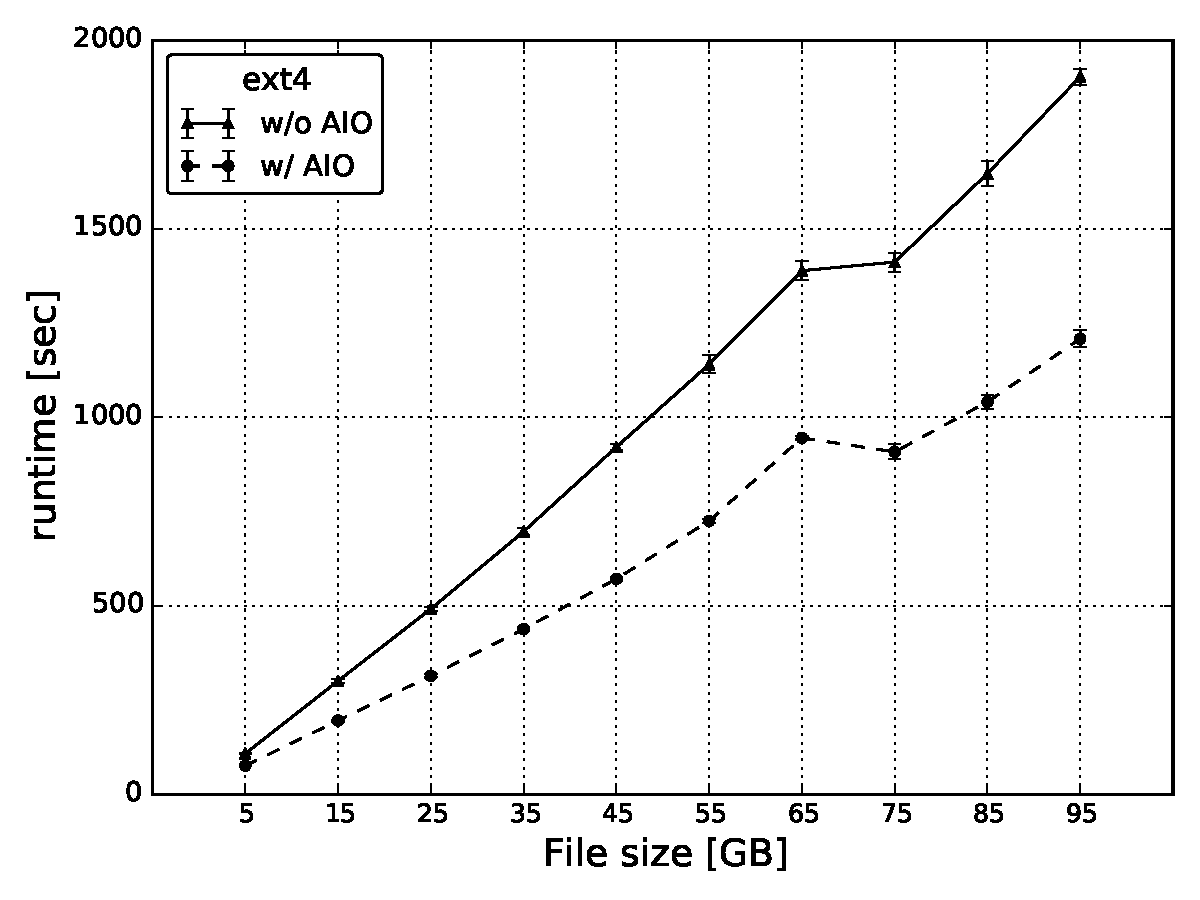
\includegraphics[width=\textwidth]{figures/SC2015/ROOT/separate_plots/test_cluster/ext4/runtime}
    \caption{\textit{}}
    \label{figure: ext4_1}
  \end{subfigure}
  \begin{subfigure}[t]{0.32\textwidth}
    \centering
    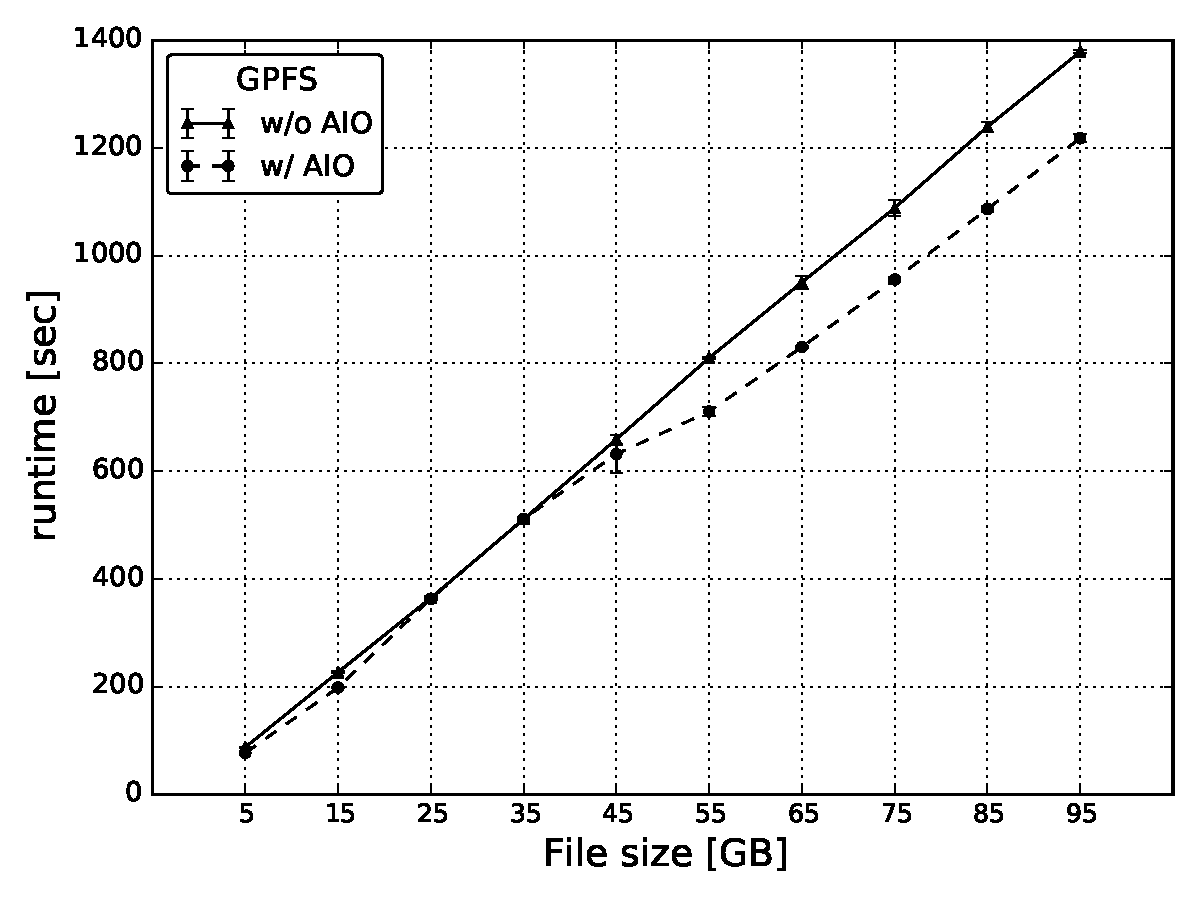
\includegraphics[width=\textwidth]{figures/SC2015/ROOT/separate_plots/test_cluster/gpfs/runtime}
    \caption{\textit{}}
    \label{figure: gpfs_1}
  \end{subfigure}
  \begin{subfigure}[t]{0.32\textwidth}
    \centering
    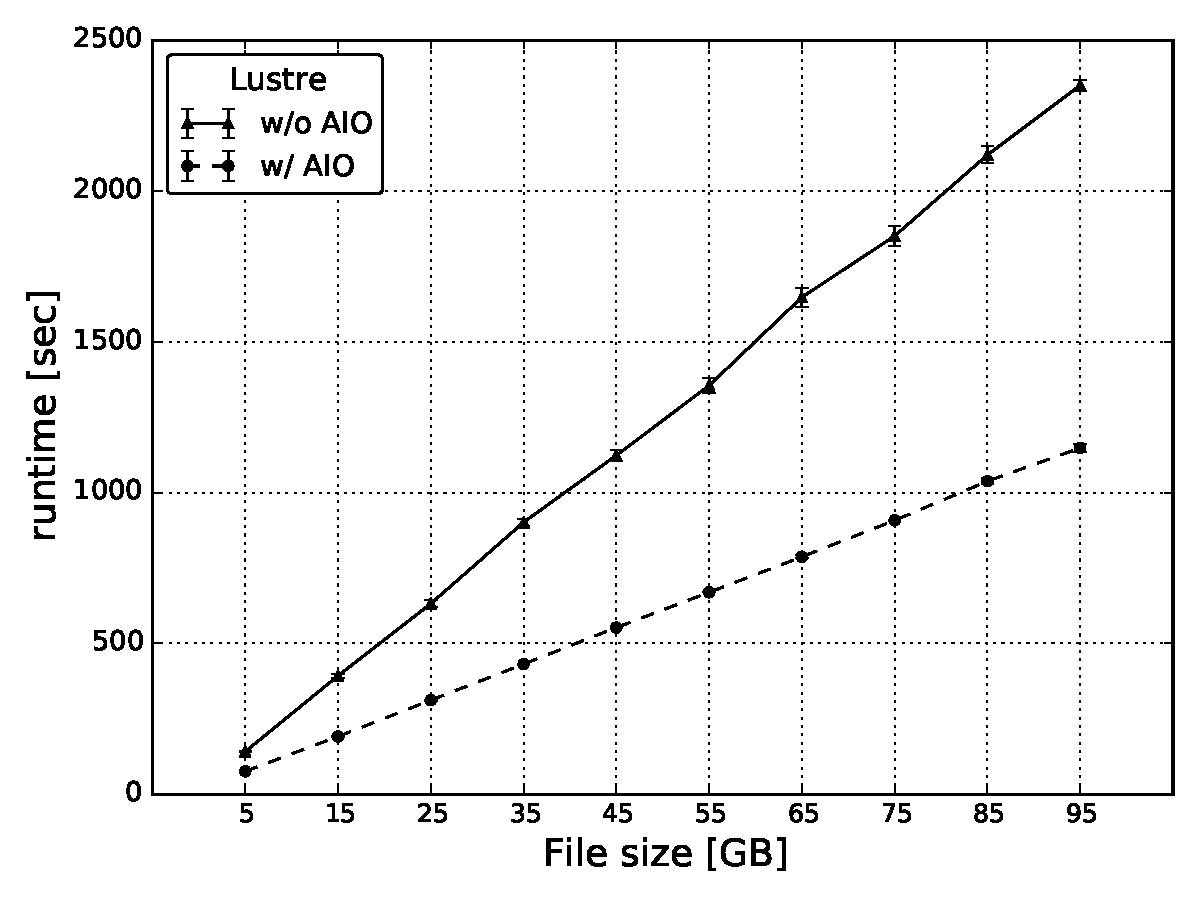
\includegraphics[width=\textwidth]{figures/SC2015/ROOT/separate_plots/test_cluster/Lustre/runtime}
    \caption{\textit{}}
    \label{figure: lustre_1}
  \end{subfigure}
  \begin{subfigure}[b]{0.32\textwidth}
    \centering
    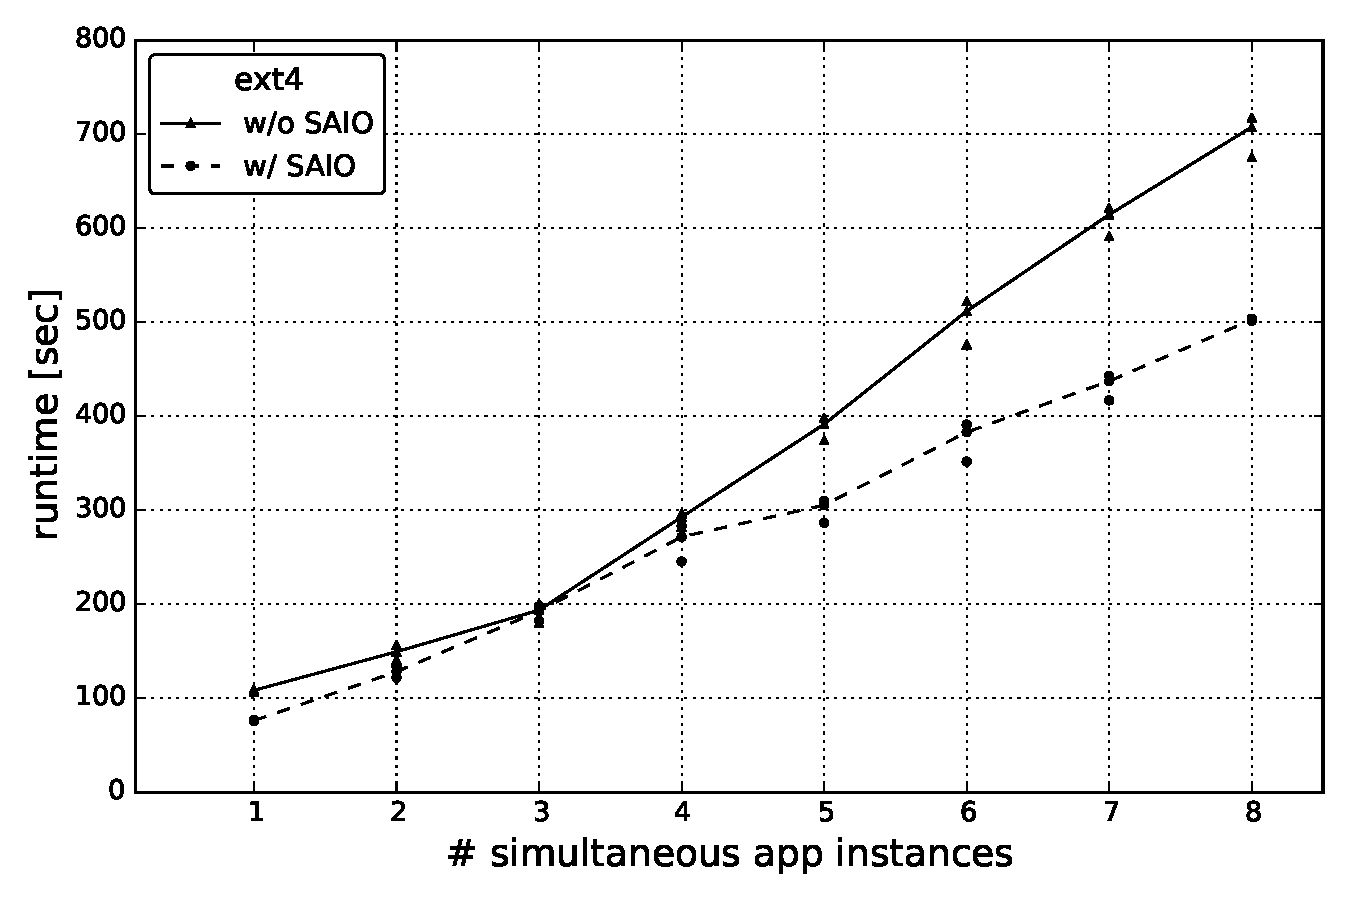
\includegraphics[width=\textwidth]{figures/SC2015/ROOT/cluster/multiple_instances/simult_instance_ext4_test_cluster}
    \caption{\textit{}}
    \label{figure: ext4_2}
  \end{subfigure}
  \begin{subfigure}[b]{0.32\textwidth}
    \centering
    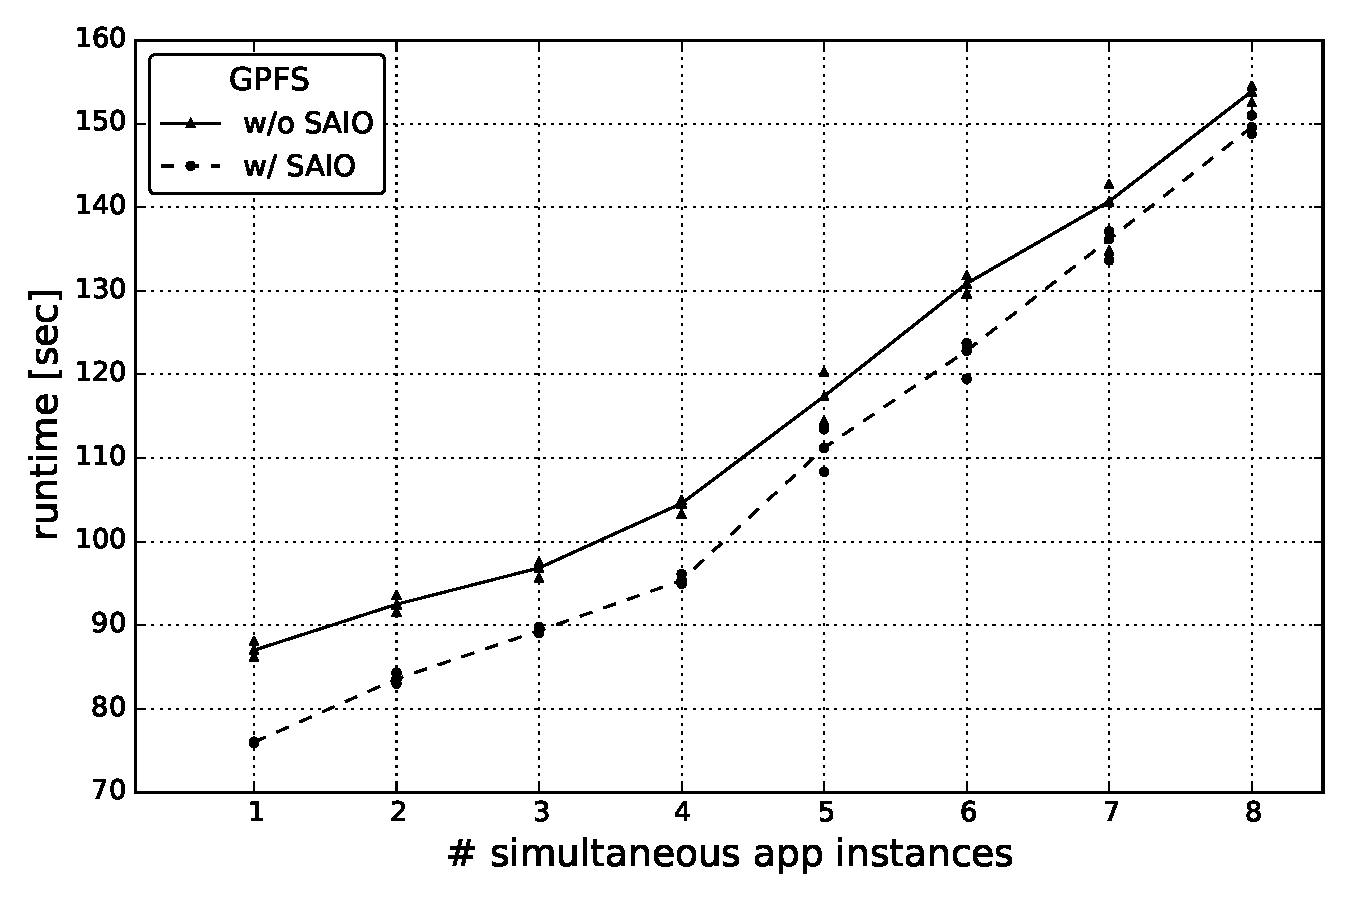
\includegraphics[width=\textwidth]{figures/SC2015/ROOT/cluster/multiple_instances/simult_instance_gpfs_test_cluster}
    \caption{\textit{}}
    \label{figure: gpfs_2}
  \end{subfigure}
  \begin{subfigure}[b]{0.32\textwidth}
    \centering
    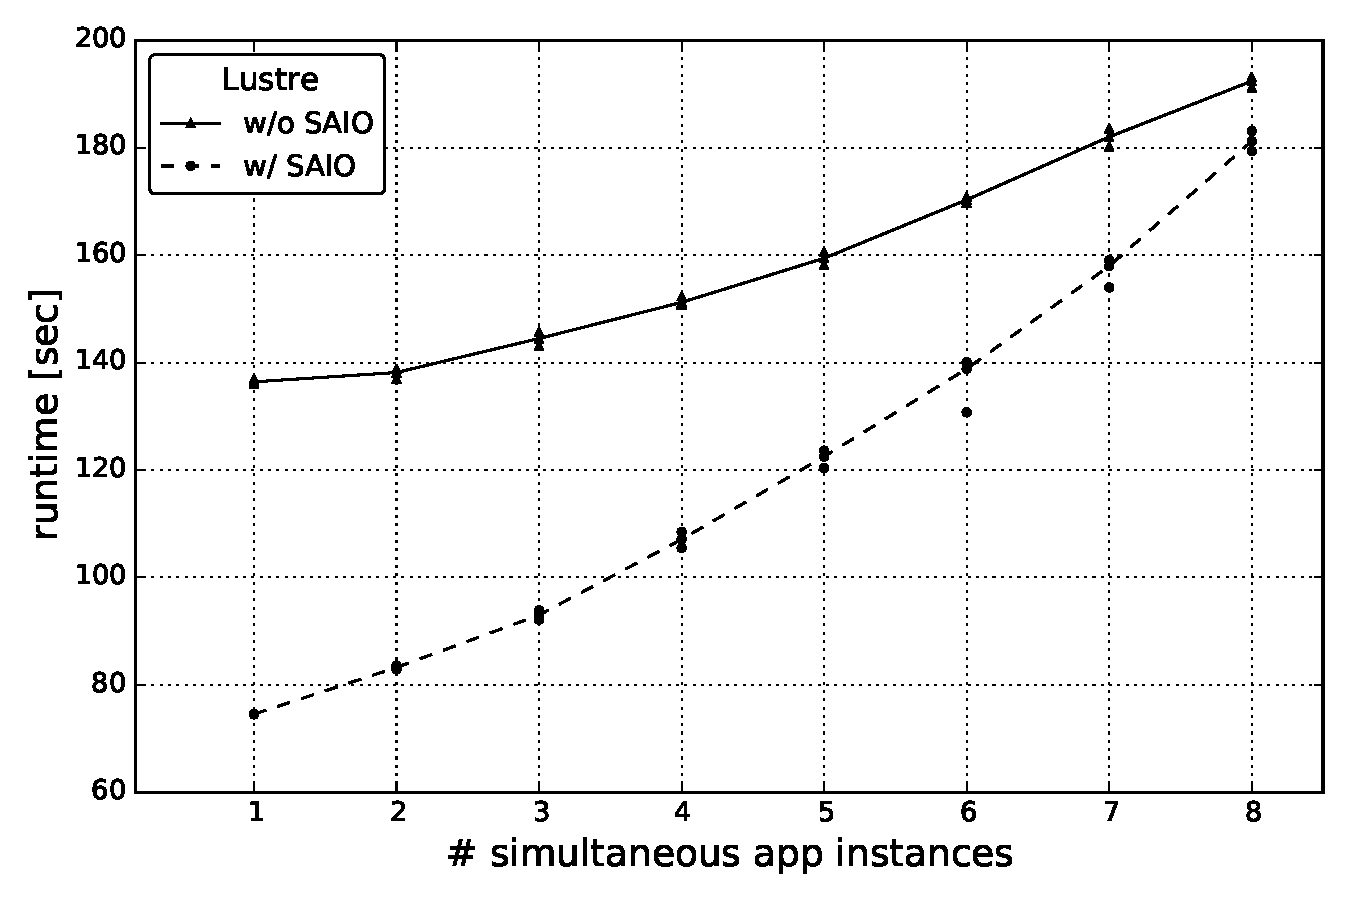
\includegraphics[width=\textwidth]{figures/SC2015/ROOT/cluster/multiple_instances/multiple_simult_procs_Lustre_testcluster}
    \caption{\textit{}}
    \label{figure: lustre_2}
  \end{subfigure}
  \caption{Running time of the ROOT application for the three file system under study using different input file sizes (\ref{figure: ext4_1},~\ref{figure: gpfs_1} and~\ref{figure: lustre_1}) and different number of instances accessing a file of 5GB (\ref{figure: ext4_2},~\ref{figure: gpfs_2} and~\ref{figure: lustre_2}).}
  \label{figure: runtime}
\end{figure*}
\begin{figure*}[!htb]
  \centering
  \begin{subfigure}[t]{0.32\textwidth}
    \centering
    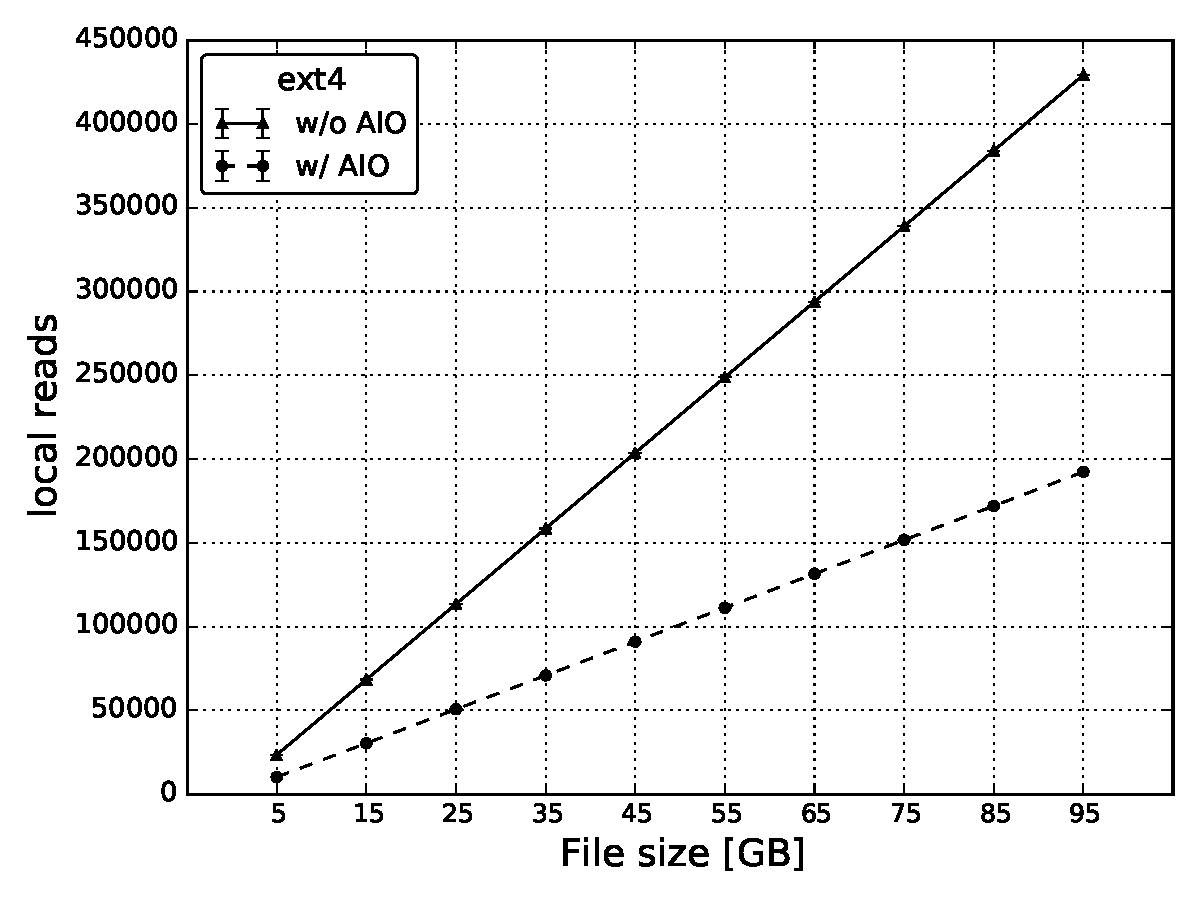
\includegraphics[width=\textwidth]{figures/SC2015/ROOT/separate_plots/test_cluster/ext4/reads}
    \caption{\textit{}}
    \label{figure: ext4_3}
  \end{subfigure}
  \begin{subfigure}[t]{0.32\textwidth}
    \centering
    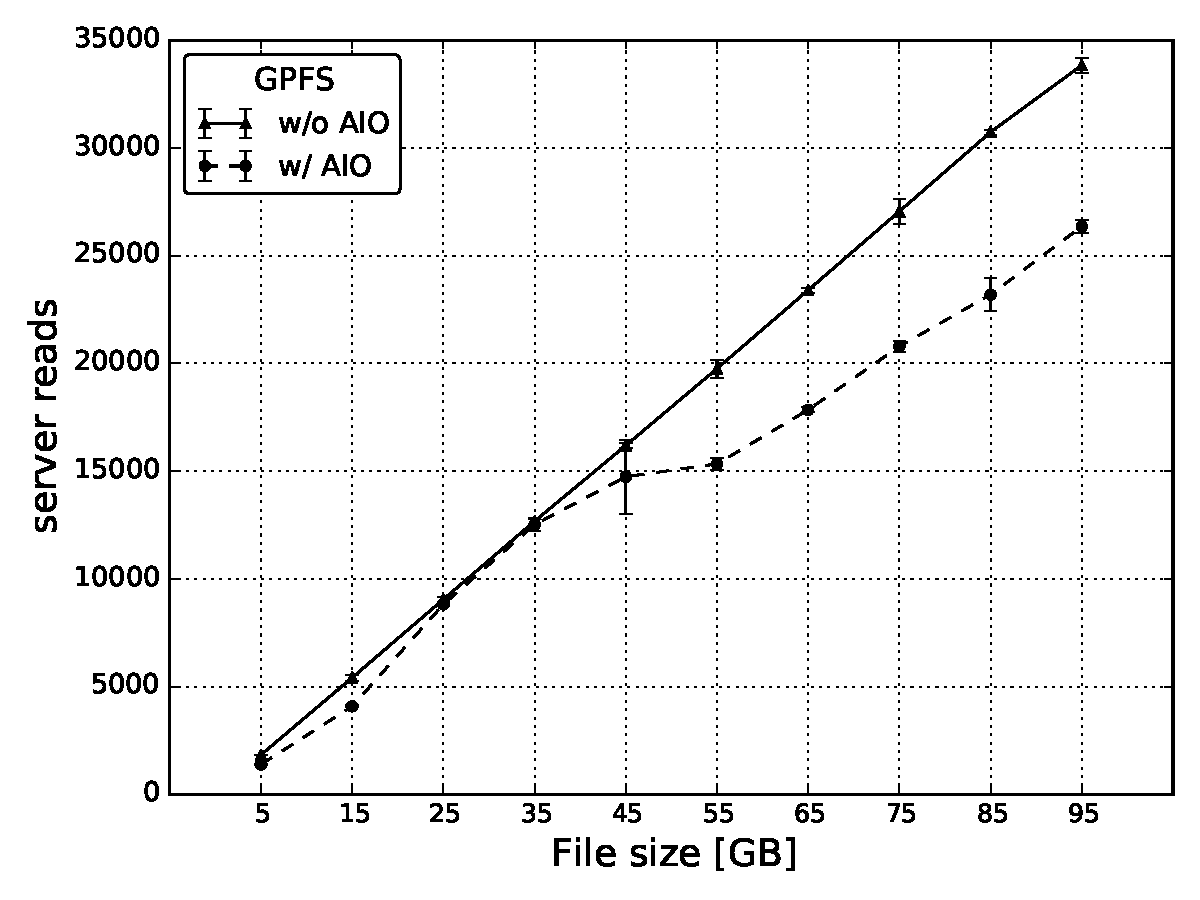
\includegraphics[width=\textwidth]{figures/SC2015/ROOT/separate_plots/test_cluster/gpfs/server_reads}
    \caption{\textit{}}
    \label{figure: gpfs_3}
  \end{subfigure}
  \begin{subfigure}[t]{0.32\textwidth}
    \centering
    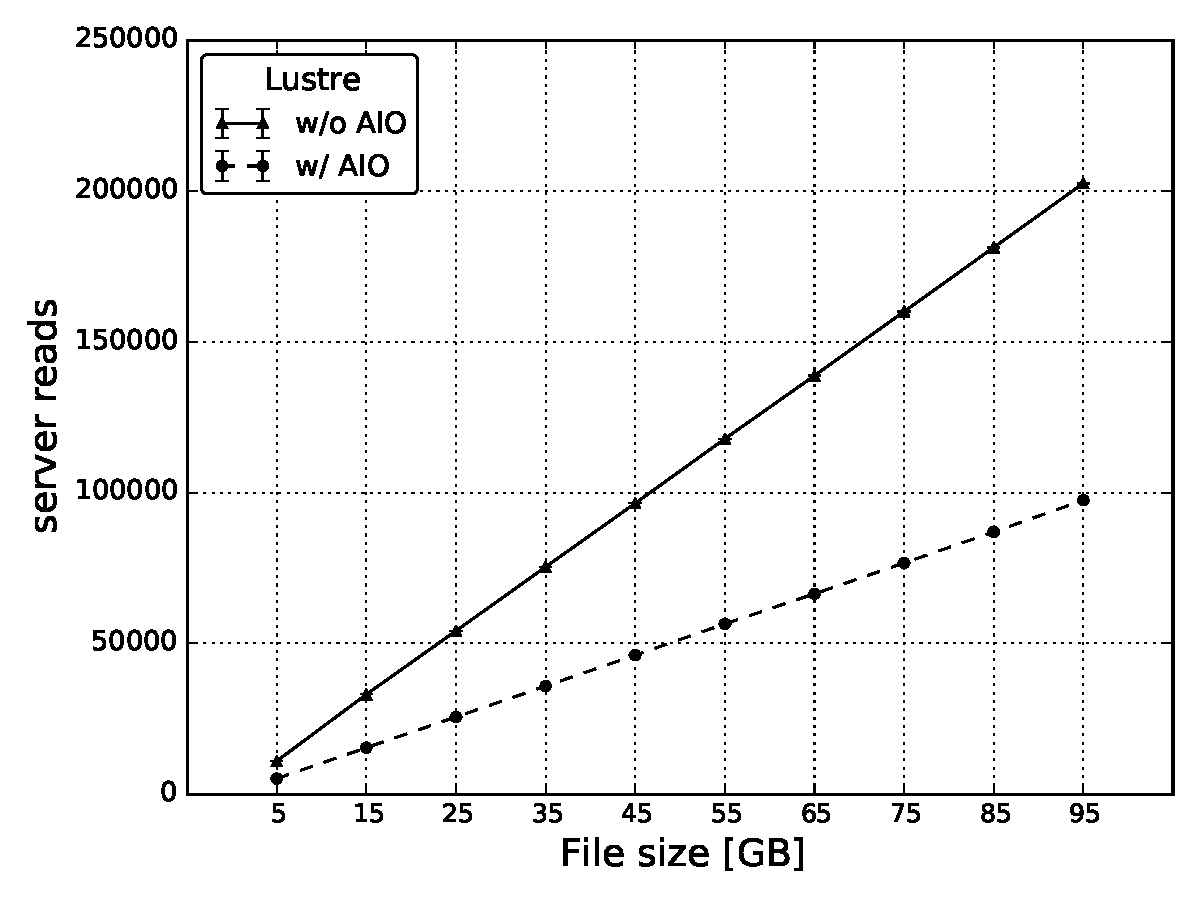
\includegraphics[width=\textwidth]{figures/SC2015/ROOT/separate_plots/test_cluster/Lustre/server_reads}
    \caption{\textit{}}
    \label{figure: lustre_3}
  \end{subfigure}
  \begin{subfigure}[b]{0.32\textwidth}
    \centering
    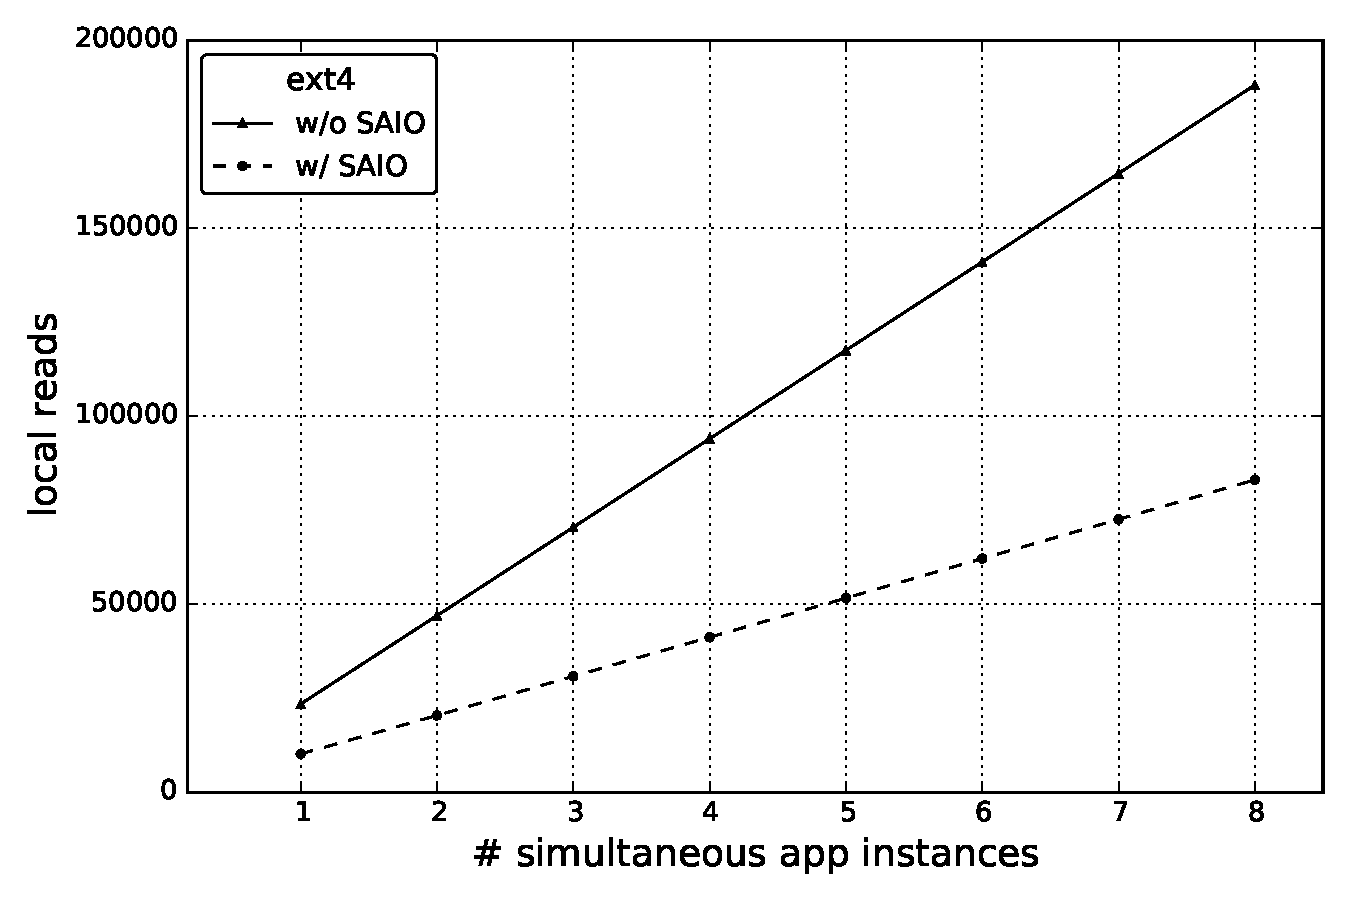
\includegraphics[width=\textwidth]{figures/SC2015/ROOT/cluster/multiple_instances/reads_simult_instance_ext4_test_cluster}
    \caption{\textit{}}
    \label{figure: ext4_4}
  \end{subfigure}
  \begin{subfigure}[b]{0.32\textwidth}
    \centering
    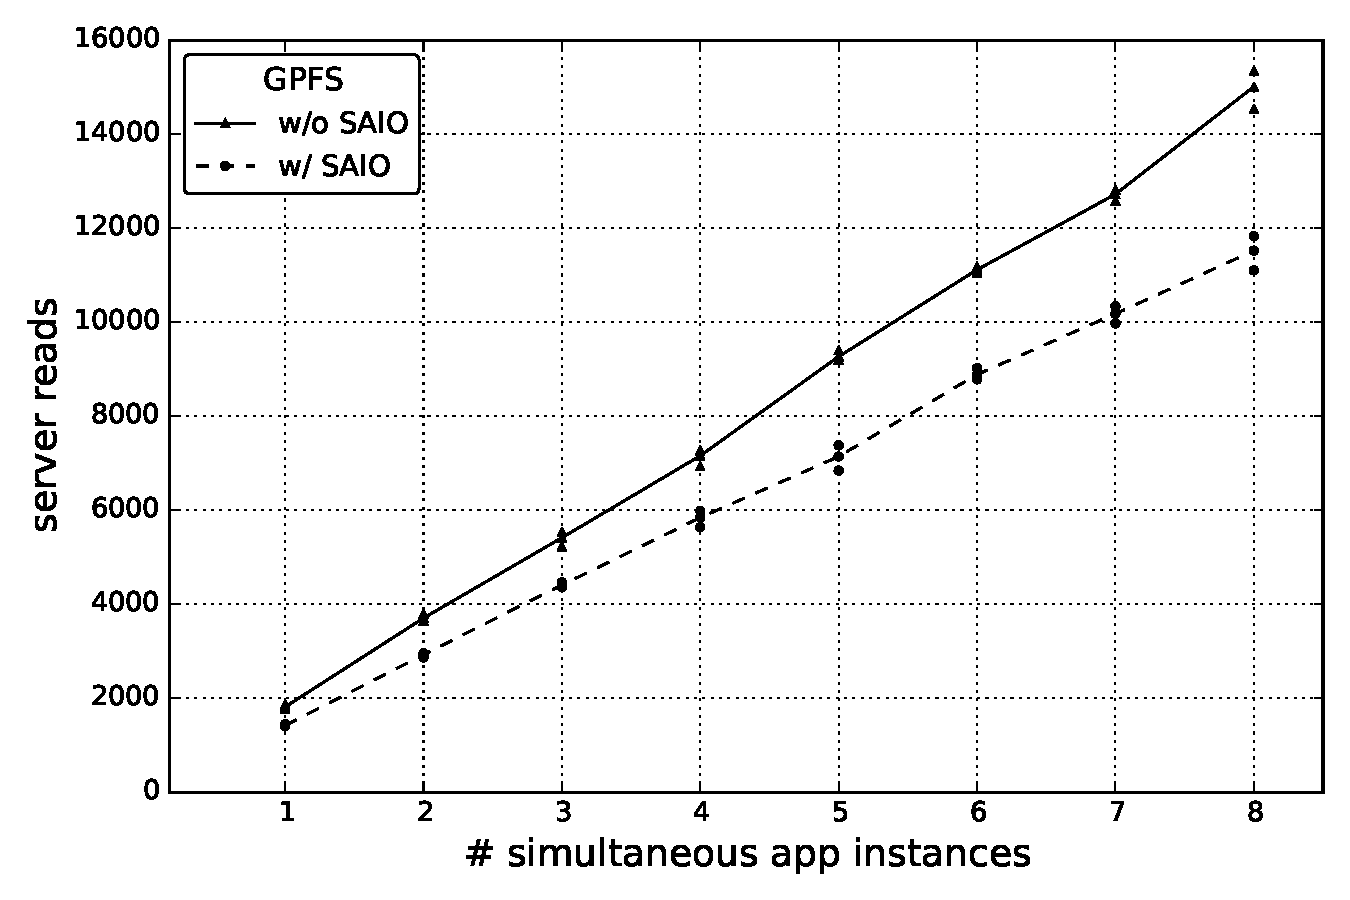
\includegraphics[width=\textwidth]{figures/SC2015/ROOT/cluster/multiple_instances/reads_simult_instance_gpfs_test_cluster}
    \caption{\textit{}}
    \label{figure: gpfs_4}
  \end{subfigure}
  \begin{subfigure}[b]{0.32\textwidth}
    \centering
    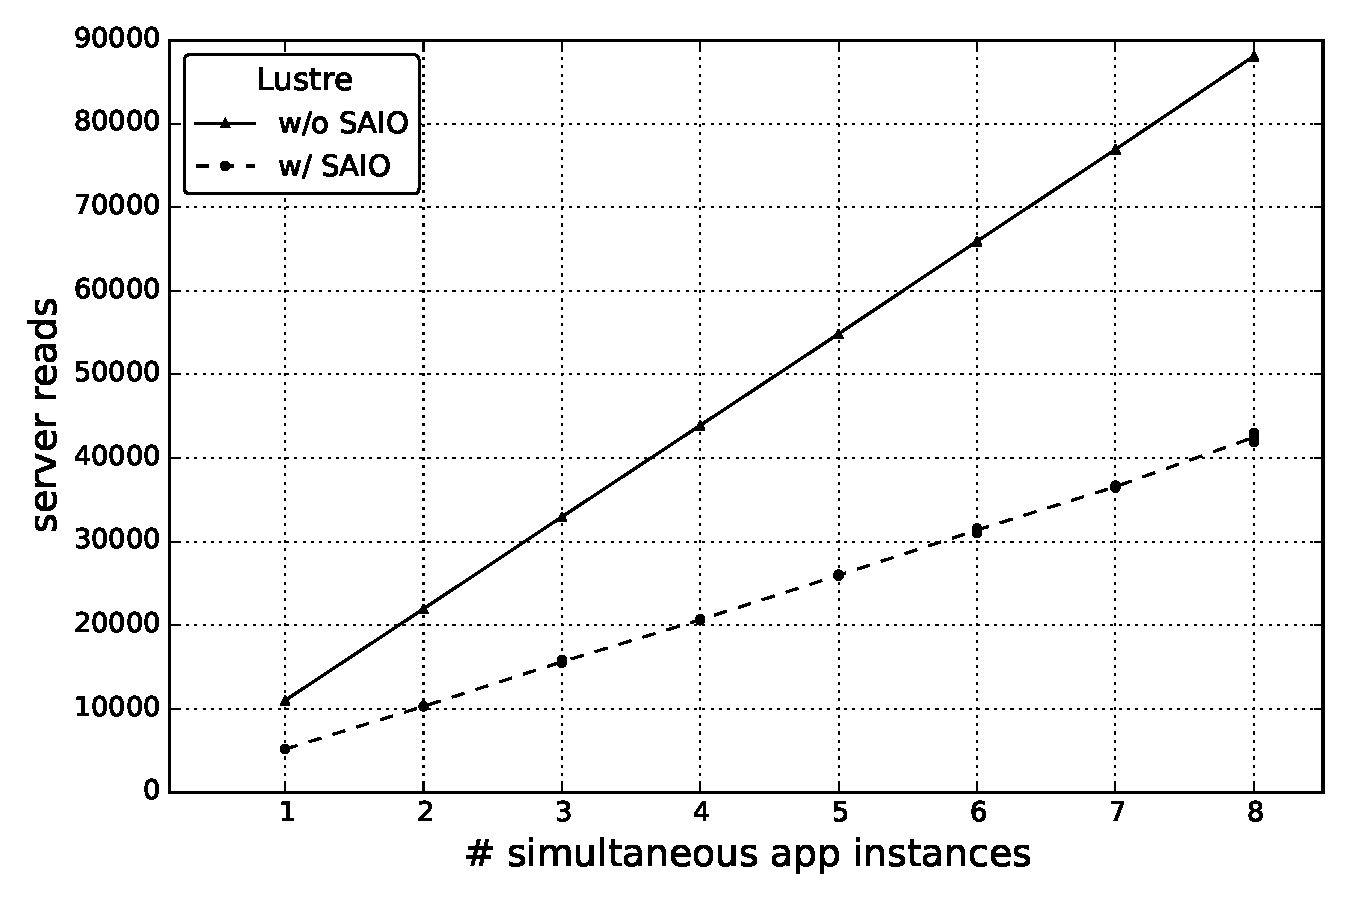
\includegraphics[width=\textwidth]{figures/SC2015/ROOT/cluster/multiple_instances/reads_multiple_simult_procs_Lustre_testcluster}
    \caption{\textit{}}
    \label{figure: lustre_4}
  \end{subfigure}
  \caption{Reads processed by local ext4, GPFS and Lustre I/O servers for various input file sizes (\ref{figure: ext4_3},~\ref{figure: gpfs_3} and~\ref{figure: lustre_3}) and multiple instances of ROOT accessing a file of 5GB (\ref{figure: ext4_4},~\ref{figure: gpfs_4} and~\ref{figure: lustre_4}).}
  \label{figure: read}
\end{figure*}

As far as Figures~\ref{figure: ext4_2},~\ref{figure: gpfs_2} and~\ref{figure: lustre_2} are concerned, these account for the effect of processes' concurrency on the file system. Before continuing with the discussion we have to make a note here. In our architecture, only one process per file system's client issues (through multiple \textit{Advisor Thread}s) hints on behalf of running applications. This introduces some overhead, since we have to pass the access information from the \textit{Assisted I/O library} to the \textit{Advice Manager}, but has the advantage of better coordinating accesses to the same file from multiple processes. Nevertheless, we found that in the case of GPFS, despite the fact of having multiple \textit{Advisor Thread}s, only one process among the many was receiving a benefit from the prefetching hints. The reason is that GPFS seems to have the restriction of hinting only one file per process. For this reason, we developed another variant of MERCURY in which the AIO library, now renamed \textit{Self Assisted I/O library} (SAIO), internally provides the creation and the handling of multiple \textit{Advisor Thread}s. Looking at the figures generated with the new SAIO library we can assess the effectiveness of the prefetching hints for the three file systems considered. In particular, Lustre provides the best runtime improvements compared to the case in which no hints were used. GPFS shows a more contained improvement since the I/O time is already small compared to Lustre and ext4. Finally, ext4 can really benefit from prefetching hints especially for high process counts. Overall, excluding ext4, when we increase the number of processes the runtime improvements shrink. This is probably due to the saturation of the file system client bandwidth.

%Figure~\ref{figure: exec_time_comparison} shows the execution time of the target application in both clusters. As already mentioned, for the experiments we tailored a configuration file in order to fit the target I/O pattern. Additionally, we also used a configuration file containing only a `WillNeed' section covering the whole file. In this last case the \textit{Advisor Thread} moves from the beginning towards the end of the file, prefetching \texttt{GPFS\_MAX\_RANGE\_COUNT} blocks at a time, following the application I/O profile (sliding window prefetch). This is intended to evaluate the relationship between costs and benefits when building a complex configuration file, instead of using a simple one that describes the general I/O behaviour of the application. %We show that a perfectly tailored config file can give better performance than a simple one. On the other hand the complexity and the effort required to build it increase.   

%\begin{figure}[!htb]
%  \centering
%  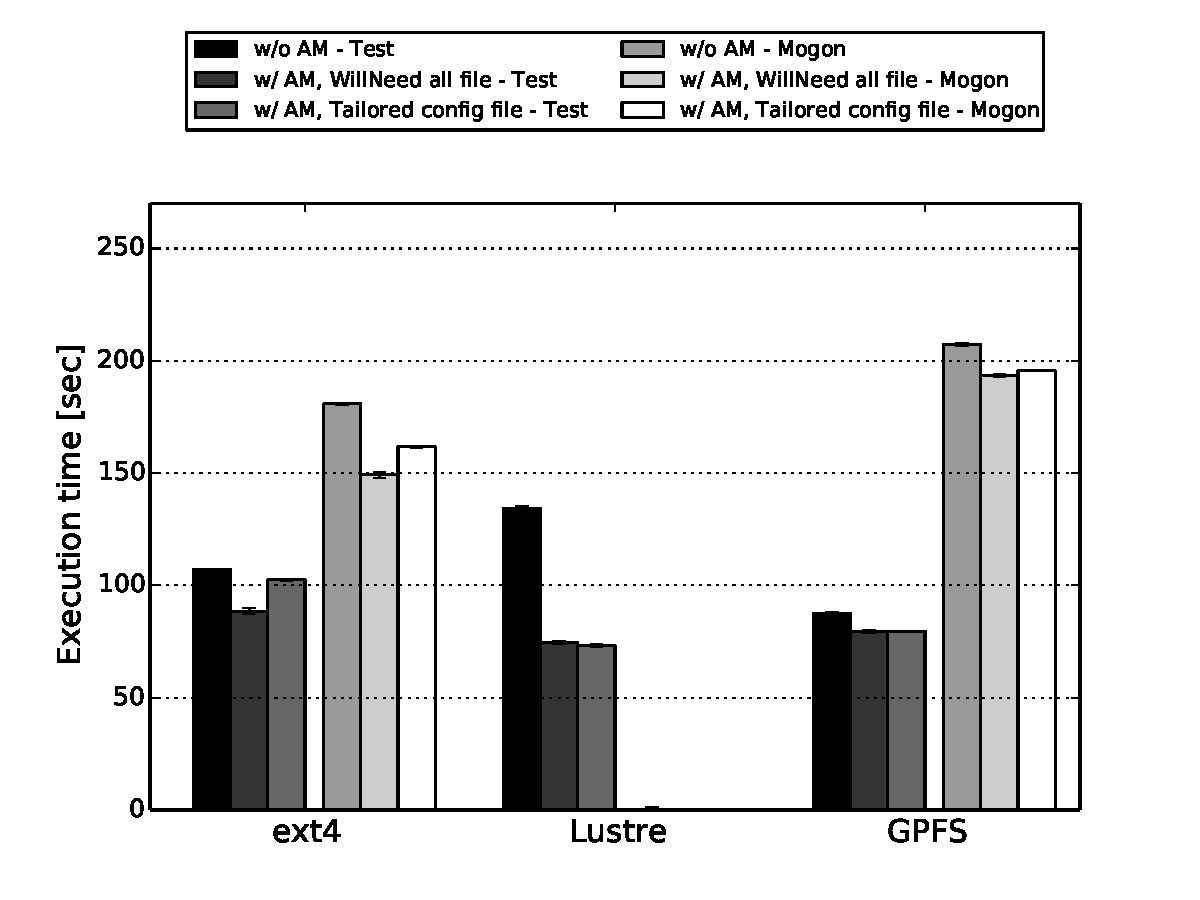
\includegraphics[width=0.44\textwidth]{figures/exec_time_comparison}
%  \caption{Execution time of the target application on the test cluster and on the `Mogon' cluster for the different available file systems.}
%  \label{figure: exec_time_comparison}
%\end{figure}

%As we can see, when the \textit{Advice Manager} is used to generate the proper hints the execution time can always be reduced. In the best case, on the test cluster this reduction is 44\% (60 seconds) for Lustre, 9\% (8 seconds) for GPFS and 17\% (19 seconds) for ext4. The big difference between Lustre and the other file systems is due to Lustre performing very poorly with the specific type of I/O pattern used (small random reads). As a result, the impact of I/O on the total time, as well as the corresponding reduction, are large compared to the other two cases. For `Mogon', we can save up to 6\% (14 seconds) of the execution time on GPFS and up to 9\% (22 seconds) on ext4. This reduction is particularly significant since in a production environment resources are highly valuable. With our approach we can reduce the application requirement of system resources (I/O and CPU time) making them available to other applications. 

%Finally, in the test cluster we can observe that using a single `WillNeed' section covering the whole file on GPFS performs equally as the tailored configuration file. In comparison ext4 performs better with the simple configuration file, while for Lustre there is no significant difference between the two cases. 
%The reason, as already mentioned, is that if the configuration file is not tailored properly GPFS may release blocks of the file that will be accessed later by the application causing cache misses and therefore degrading the performance. 
%In the `Mogon' cluster there is no visible difference in the performance of these two test cases for GPFS.
%, because the tests were not performed at the same time and the load level of the file system may have changed significantly in the meanwhile. 
%Also in this case, ext4 on Mogon gives its best performance for the configuration covering the whole file, 4\% reduction (10 seconds) compared to the tailored configuration. 

%In conclusion, here we showed that for the specific I/O pattern exposed by the target application, a perfectly tailored configuration file does not necessarily give the best performance in terms of execution time of the application. On the other hand, a configuration file that covers the whole file, capturing the general behaviour of the application can still give significant improvements, with the additional benefit that it is general enough to serve any input file and requires no time to be built.   
%The results shown in Figure~\ref{figure: fullnode_mogon_exectime} are more relevant, as they were obtained on a production cluster. In fact, saving a few seconds from an applications runtime has a large impact because it means that we use less CPU time accross the cluster, allowing more users to run their applications and increasing job throughput for the administrator.
%In Figure~\ref{figure: fullnode_mogon_exectime} we clearly see that on Mogon there is a wide variation in the execution times for the local file system when we run with and without the \textit{Advice Manager} and this effect doesn't not change for the different configurations tested. To be more specific, the improvement in the runtime is 8.6$\%$ and 12$\%$ respectively for the local file system and for GPFS.

\subsection{Read Request Rate}
\label{subsec: reads}
Figure~\ref{figure: ext4_3},~\ref{figure: gpfs_3} and~\ref{figure: lustre_3} report the number of read requests accounted for by the different file systems under study. In the specific, the figures show how the number of reads at the I/O server side for both GPFS and Lustre can be substantially reduced with our approach. This has a significant impact in HPC cluster in which the file system may be accessed by many thousand of processes at the same time. Reducing the number of requests for an application can increase the number of IOPS available for others. This result is also confirmed for multiple instances of the `ROOT' application running concurrently (Figure~\ref{figure: ext4_4},~\ref{figure: gpfs_4} and~\ref{figure: lustre_4}).
%We now report the effect that hints have on the number of reads. To measure this we used three different tools, according to the file system under test. For ext4 we monitored the individual disk involved, acquiring the statistics from the `sysfs' file system. For Lustre we used the \textit{collectl}~\cite{collectl} tool which permits us to measure the reads processed by the OSTs in a simple way. Finally, for GPFS we used the \textit{mmpmon} tool mentioned before, which measures the reads on the file system client side.
%TODO reference for collectl? http://collectl.sourceforge.net/ is there an introductory paper for it?

%Figure~\ref{figure: reads_final_comparison} shows the obtained results in both clusters. As we can see, in the test cluster there is a consistent improvement when the \textit{Advice Manager} is used. For ext4 and Lustre we observe a reduction of circa 50\% in the number of  read requests, as many of the I/O requests are satisfied by the relevant caches populated by the \textit{Advice Manager}. For GPFS the number of read requests processed by the NSD server was reduced by up to 84\% (from 4697 to 762).

%\begin{figure}[!htb]
%  \centering
%  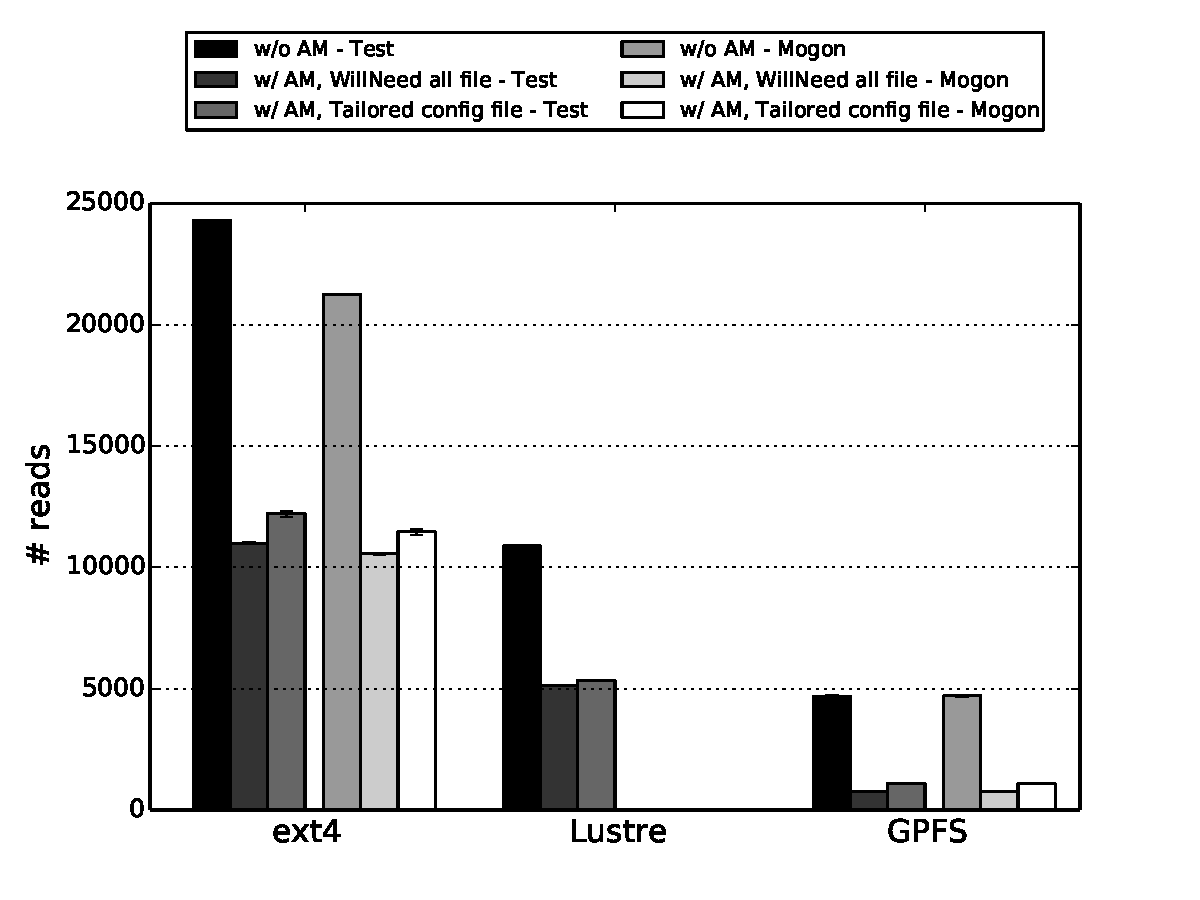
\includegraphics[width=0.44\textwidth]{figures/reads_final_comparison}
%  \caption{Number of read operations accounted for by the different file systems on the test cluster and on the `Mogon' cluster.}
%  \label{figure: reads_final_comparison}
%\end{figure}

%As for the execution time, in this case we can notice that there is a small difference between the number of reads obtained with the tailored configuration file and the configuration file covering the whole file. In particular, the last configuration file performs better than the first one since in this case the implementation prefetches more data.
%The reason for this is that while the last one covers the whole file, the first leaves some small portion of the file uncovered. This was a choice we made to simplify the configuration file. 

%TODO: so its incomplete - you turn the read ahead system off part way through the test?

%The presented results are particularly relevant in the case of highly parallel environments where many applications are using the file system at the same time. Indeed, in this case by reducing the number of requests that the file system has to handle for every file, we can increase the number of IOPS available for other applications and therefore improve the overall performance. 

%\subsection{Effect of Background Processes}
%\label{subsec: bkg_procs}
%One interesting thing to look at is the effect of other processes and applications using resources on the file servers. In this respect, it only make sense to investigate such a scenario for distributed and parallel file systems. For this reason, we show results for Lustre and GPFS on the test clusters. Concerning Mogon, the results for the execution time and the number of read requests processed already include the effect of many processes requesting resources from the file servers. Although we reserved a complete node with 64 cores, there are many other nodes running a multitude of different applications that are putting load on the file servers. When looking at the results it should be no surprise that the execution times of the application running on a clean test environment and on a production cluster differ.

%Table~\ref{table: runtime_bkg} reports the results for execution time and number of reads under heavy load of the file systems by another 60 processes. These processes run on the three free nodes of the test cluster (those not running the application) and each of them continuously generates random reads for 20 files, (for a total of 60 files). In this case we can notice that practically there is no difference between a tailored configuration file and a configuration file covering the whole file, aligning with the results showed in Figure~\ref{figure: exec_time_comparison} for `Mogon' and test cluster. We can also notice that for GPFS the number of read operations does not change. The reason is that \textit{mmpmon} only measures statistics on the file system client side. For Lustre, on the other hand, we also see the contribution of the other processes accessing the file system since we measure the reads at the OSTs.  

%\begin{table*}[!ht]
%\caption{Test cluster's results under heavy loaded file systems.}
%\centering
%\resizebox{1\textwidth}{!}{\begin{minipage}{\textwidth}
%\begin{tabular}{  l  c  c  c  c }
%\toprule
% & \multicolumn{2}{c}{Lustre} & \multicolumn{2}{c}{GPFS} \\
%   & Exec time [sec] & \# reads & Exec time [sec] & \# reads \\
%   \midrule
%   w/o AM & 148.85$\pm$1.47 & 1615623$\pm$11111 & 104.35$\pm$1.48 & 4675$\pm$30 \\ 
%   w/ AM Tailored config & 81.82$\pm$1.17 & 1324290$\pm$4845 & 81.38$\pm$0.46 & 1089 \\ 
%   w/ AM WillNeed all file & 80.48$\pm$0.47 & 1320422$\pm$3476 & 79.72$\pm$0.41 & 762 \\ 
%\bottomrule  
%\end{tabular}
%\end{minipage}}
%\label{table: runtime_bkg}
%\end{table*} 

%\subsection{Overhead}
%\label{subsec: overhead}
%As a final test, we evaluated the overhead introduced by our advice infrastructure prototype to the application. This was done by creating a configuration file that contains no advice for the input file. Correspondingly, the \textit{Interposing I/O Library} intercepts the read calls of the application and forwards them to the \textit{Advice Manager}, but this time it does not generate any hints`. The result is that the application runs normally with the additional overhead of the interprocess communication between \textit{Interposing I/O Library} and \textit{Advice Manager}. With this experiment we observed 0.68\% overhead on the test cluster for Lustre and 3\% for GPFS. Since the communication overhead is constant, the impact on GPFS is bigger being the execution time on GPFS smaller than Lustre. 
%So here we report our findings on the test cluster for Lustre and GPFS. What we do in this case is to try to put load on the respective servers from a number of processes running on three independent nodes, (not those running the application). In each of these nodes we start in parallel 30 instances of a program which performs random reads from specified files on the shared file system. After the network traffic to the file system servers has stabilised, we start our application and its associated monitoring. Table~\ref{table: runtime_bkg} reports the corresponding execution time results. 

%\begin{table*}[!ht]
%\caption{}
%\centering
%%\resizebox{1\textwidth}{!}{\begin{minipage}{\textwidth}
%\begin{tabular}{  l  c  c  c  c  c  c }
%\toprule
% & \multicolumn{3}{c}{Lustre} & \multicolumn{3}{c}{GPFS} \\
%   \footnotesize & Exec time [sec] & \# reads & overhead [\%] & Exec time [sec] & \# reads & overhead [\%]\\
%   \midrule
%   w/o AM & 148.85$\pm$1.47 & 1615623$\pm$11111 & - & 104.35$\pm$1.48 & 4675$\pm$30 & - \\ 
%   w/ AM Tailore config & 81.82$\pm$1.17 & 1324290$\pm$4845 & 0.68 & 81.38$\pm$0.46 & 1089 & 3.06 \\ 
%   w/ AM WillNeed all file & 80.48$\pm$0.47 & 1320422$\pm$3476 & - & 79.72$\pm$0.41 & 762 & - \\ 
%\bottomrule  
%\end{tabular}
%\end{minipage}}
%\label{table: runtime_bkg}
%\end{table*} 

%%Since our advice infrastructure is meant to be used in everyday work, it's important to assess the overhead it introduces to the normal execution of the application.
%%We already saw that the improvement and the benefit can be big, both in the reduction of the execution time and of the number of reads the the storage system will have to handle.
